\documentclass[11pt,a4paper, dvipsnames]{article}
\usepackage{tmh}
\renewcommand{\familydefault}{\sfdefault}
\usepackage[scaled]{helvet}

\renewcommand{\phi}{\varphi}
% Default fixed font does not support bold face
\DeclareFixedFont{\ttb}{T1}{txtt}{bx}{n}{10} % for bold
\DeclareFixedFont{\ttm}{T1}{txtt}{m}{n}{10}  % for normal

% Custom colors
\usepackage{xcolor}
\definecolor{deepblue}{rgb}{0,0,0.5}
\definecolor{deepred}{rgb}{0.6,0,0}
\definecolor{deepgreen}{rgb}{0,0.5,0}
\usepackage{framed}
\usepackage{listings}

% Python style for highlighting
\newcommand\pythonstyle{\lstset{
        language=Python,
        basicstyle=\footnotesize\ttm,
        otherkeywords={self},             % Add keywords here
        keywordstyle=\ttb\color{deepblue},
        emph={MyClass,__init__},          % Custom highlighting
        emphstyle=\ttb\color{deepred},    % Custom highlighting style
        stringstyle=\color{deepgreen},
        frame=tb,                         % Any extra options here
        showstringspaces=false            % 
}}


% Python environment
\lstnewenvironment{python}[1][]
{
    \pythonstyle
    \lstset{#1}
}
{}

% Python for external files
\newcommand\pythonexternal[2][]{{
        \pythonstyle
        \lstinputlisting[#1]{#2}}}

% Python for inline
\newcommand\pythoninline[1]{{\pythonstyle\lstinline!#1!}}

\usepackage[many]{tcolorbox}
\usepackage{marginnote}

\newtcolorbox{boxnote}[1][]{
    width=\textwidth,
    fonttitle=\bfseries,
    breakable,
    fonttitle=\bfseries\color{Brown},
    colframe=Melon,
    colback=Melon!10
    #1}

\newcounter{mynote}
\newtcolorbox[use counter=mynote]
{mynote}[1][]
{title=Note~\thetcbcounter,
    width=5cm,
    left=0pt,
    right=0pt,
    fonttitle=\bfseries\color{Brown},
    colframe=Melon,
    colback=Melon!10,
    #1
}    

\begin{document}
    \mytitle{Particle Models}
    \section{Model Implementation}
        The main difficulty in moving from the space homogenous to the two dimensional case is calculating the heterogeneity for every particle.
        
        The problem term is:
        \begin{equation}\label{interaction}
            G\left(\frac{\frac{1}{N}\sum_{j=1}^N v_t^{j,N}\varphi(x^{j,N}_t-x^{i,N}_t)}{\frac{1}{N}\sum_{j=1}^N \varphi(x^{j,N}_t-x^{i,N}_t)}\right).
        \end{equation}
        Let's unpack this piece by piece, and discuss their implementation. The herding function $G$, is identical to before, with a new option \texttt{G\_Garnier}, corresponding to the variable well-depth function given in Garnier's paper:
        $$G(u) = \frac{h+1}{5}u - \frac{h}{125} u^3$$
        Calculating the interaction is more difficult computationally. For every particle we must calculate the distance to every other particle in the system. A first implementation is shown below.

        \begin{python}
x_curr = x[n] #Particles' current positions
   for particle, position in enumerate(x_curr):
       dist = np.abs(x_curr - position)
       interaction = phi(np.minimum(L-dist, dist))
       weighted_avg = np.sum(v[n, ] * interaction)
       scale = np.sum(interaction)
       interaction_vector[particle] = weighted_avg / scale
        \end{python}
        For each particle in the system, we calculate the difference between all positions and the particle position, modulo the length of the domain. This is equivalent to $\min(x_i-x_j, L-(x_i-x_j))$ but requires less operations. The implementation here should be quick, as it exploits NumPy's ability to broadcast arrays of different sizes. The state of the system is then updated as before.
        \begin{python}
x[n + 1,] = (x[n,] + v[n,] * dt) % (L)  # Restrict to torus
v[n + 1,] = (v[n,] - (v[n,] * dt) + G(interaction_vector) * dt
            + D*np.sqrt(dt) * normal(size=particles))
        \end{python}
        
        \begin{boxnote}
            Should the interaction include the current particle? As it's written, the particle interacts with itself. Could be attributed to some sort of ``inertia''. In the case of one particle, \eqref{interaction} becomes  
            \[ G\left(\frac{v^1_t\phi(0)}{\phi(0)}\right) = G(v^1_t).\]
            The equation of motion for this particle is then 
            \[\dif v^1_t = -v^1_t \dif t + G(v^1_t) \dif t +\sqrt{2\sigma}\dif W^1_t.\]
            This is very different from a free particle moving in a potential well. It will move between velocity $\pm1$, not 0 as would be expected for a free particle. \\
            \\
            Obviously this effect decreases very quickly as $N \gg 1$. Removing the particles self-interaction is not difficult.
        \end{boxnote}
        \subsection{Differences in Garnier's Model}\label{garnierdiff}
            Garnier's model differs in three ways: the scaling of the interaction, the size of the spatial domain and the diffusion coefficient. The diffusion coefficient here is $\frac{\sigma^2}{2}$ instead of just $\sigma$. No changes to the implementation are necessary here, other than minor plotting changes. The potential function is also easily implemented. Changing the length of the domain from $2\pi$ doesn't materially affect anything as it can just be scaled back to the unit circle. I can't see any reason for using a longer domain, other than it avoiding a call to NumPy. The only difference that may have an effect is the scaling of the interaction. Rather than counting the number of particles that contributed to the interaction, the total number of particles is used. This difference is mentioned in Section 8, where they conclude that it will have an effect on the critical diffusion value that makes the order states stable. As far as I can tell no simulations were done to confirm this.
            \begin{boxnote}
                Scaling by $N$ will reduce the input to $G$, biasing the velocity towards 0. Is this why in low noise we see velocity away from the expected value? Try running for with each denominator -- still get cluster, but avg vel is much closer to where it is expected to be?
            \end{boxnote}
            
    \section{Sanity Checks}
        To check this implementation is working as expected, we can exploit the analysis and the earlier code. Things to check:
        \begin{enumerate}
            \item If $\phi\equiv 0$, does the interaction return zero?
            \begin{enumerate}
                 \item  Does the system converge to $\mathcal{N}(0,\sigma)$?
            \end{enumerate}
            \item If $\phi \equiv 1$, does the \texttt{interaction\_vector} return the average velocity?
            \begin{enumerate}
                 \item  Does the system converge to $\mathcal{N}(\pm \xi,\sigma)$, where $G(\xi)=\xi$? 
            \end{enumerate}
            \item If $\phi = I_{[0,1]}$ and we place say 5 particles on the torus deterministically, does the code return the same as we calculate by hand?
        \end{enumerate}
        First we will verify the interaction calculations, before testing convergence.
        
        \subsection{Interaction Checks}
        The test functions are contained in \verb|test_sanity.py|. All tests take as input a random vector of length 1000 as simulated data. When $\phi \equiv 0$, we simply check every entry is zero. For $phi \equiv 1$, we expect the interaction to be the mean of all velocities. The functions \verb|test_zero()| and \verb|test_ones()| assert this. The final hand check of $\phi = I_{[0,1]}$ is in \verb|test_hand()|.
        
        \subsection{Convergence Checks}
        To assess the convergence, we can use firstly a visual check using a histogram, then the Kullback-Leibler divergence for normal and uniform distributions and the centred $L_2$ discrepancy for the spatial distribution.
        
        \begin{framed}
            \textbf{Aside: Calculating KL and CL2}\\
            The Kullback-Leibler divergence already exists in Python as \texttt{scipy.stats.entropy()}. The centred L2 discrepancy however does not. It is quite slow to calculate as it involves a double sum, not sure if there's any way around that. Trying to be Pythonic and using \texttt{np.meshgrid} actually ended up being 4 times slower. This may be because of the size of the meshgrid, but I'm not sure.
            
            \begin{python}
def CL2_mesh(x, L=(2*np.pi)):
    n  = len(x)
    term3 = 0
    term2 = np.sum(2. + np.abs(x/L - 0.5) - np.abs(x/L - 0.5)**2)
    x_i,x_j = np.meshgrid(x,x)
    term3 = 0.5*np.sum(2+ np.abs(x_i/L - 0.5) + np.abs(x_j/L - 0.5)
         - np.abs(x_i/L - x_j/L) )
    
    CL2 = (13/12) - (term2 - term3/n)/n
    return CL2
                \end{python}
            One of the for loops has been removed here, this implementation seems to suffice.
            \begin{python}
def CL2(x, L=(2*np.pi)):
    n  = len(x)
    term3 = 0
    term2 = np.sum(2. + np.abs(x/L - 0.5) - np.abs(x/L - 0.5)**2)
    for i in range(n):
    term3 += np.sum(1. + np.abs(x[i]/L - 0.5)/2 +
        np.abs(x/L - 0.5)/2 - np.abs(x[i]/L - x/L)/2)
    CL2 = (13/12) - (term2 - term3/n)/n
    
    return CL2
                \end{python}
          Again these calculations need checking, I've done that using \verb|test_CL2()| which simulates uniform random numbers and compares their mean and variance against the theoretical CL2 values given in Garnier's paper. Running the function plots the discrepancy and mean as well as the predicted mean. 
        
        \end{framed}

    We know that if $\phi \equiv 0$ the system should converge to a Gaussian velocity with mean 0 and a uniform spatial distribution. We can compare the results here with the earlier space homogeneous system. This won't be very illuminating, as the checks on the interaction calculation seem water tight. The diffusion parameter was chosen so that $\sigma \neq \sigma^2$ and $\sigma \neq \sigma^2 / 2$, basically so that the difference between Garnier's method can be seen.
    \\
    KL divergence was 0.000643480399. CL2 discrepancy was $2.9874356 \times 10 ^{-5}$, theoretical mean is $8.333 \times 10 ^{-5}$
    
\begin{python}
particles = 2000
diffusion = 4
t,x,v = run_full_particle_system(interaction_function="Zero",
particles=particles,
D=diffusion,
initial_dist_v=np.random.normal(loc=0.5, scale=np.sqrt(2), size=particles),
T_end=100
)
\end{python}
\begin{figure}
    \centering
    \includegraphics[width=1.1\linewidth]{zeroconvergencexvhist.jpg}
    \caption{Histograms of position and velocity for no interaction. Orange shows same setup for homogeneous system. Dashed lines are theoretical stationary measure (i.e. $\mathcal{N}(0,\sigma)$ in velocity, uniform in space)}
\end{figure}


Set up for normal convergence both positive and negative with \verb|step_G| and Garnier $G$. Plots of histograms. 

\begin{python}
particles = 2000
diffusion = 4
startTime = datetime.now()
t,x,v = run_full_particle_system(interaction_function="Uniform", 
herding_function="Step"
particles=particles,
D=diffusion,
initial_dist_v=np.random.normal(loc=0.5, scale=np.sqrt(2), size=particles),
T_end=100
)
\end{python}
\begin{figure}
    \centering
    \includegraphics[width=\linewidth]{oneconvxvhist}
    \caption{Histograms of position and velocity for uniform interaction. Orange shows same setup for homogeneous system. Dashed lines are theoretical stationary measure (i.e. $\mathcal{N}(1,\sigma)$ in velocity, uniform in space). KL Divergence was $0.0023419970369$ and CL2 discrepancy was $5.3347 \times 10 ^{-5}$ with expected value $8.33\times 10^{-5}$. Convergence to $-1$ has also been checked with similar results.}
\end{figure}
Finally just to check the Garnier interaction works as expected.
\begin{python}
particles = 2000
diffusion = 4
well_depth = 6
xi = 5*np.sqrt((well_depth-4)/well_depth)
startTime = datetime.now()
t,x,v = run_full_particle_system(interaction_function="Garnier", 
herding_function="Garneir"
particles=particles,
D=diffusion,
initial_dist_v=np.random.normal(loc=0.5, scale=np.sqrt(2), size=particles),
T_end=100
well_depth=well_depth,
L=10
)
\end{python}

    \section{Garnier Figure Reproduction}
    Satisfied that the interaction is correct and the heterogeneity is included properly. To reproduce Garnier's results we should be able to just plug their parameters into our model, remembering the difference in diffusion ($\frac{\sigma^2}{2}$) and the scaling of the interaction as mention in Section \ref{garnierdiff}. I've a feeling the scaling affects the results. All axes are scaled to look exactly like Garnier's.

    \begin{figure}
        \centering
        \includegraphics[width=1.1\linewidth]{GarnierFigure2}
        \caption{Garnier Figure 2: Average velocity and CL2 discrepancy for $ h=2$ (top) and $h=4$ (bottom). This is pretty much identical to Garnier's.}
    \end{figure}

    \begin{figure}
        \centering
        \includegraphics[width=1.1\linewidth]{GarnierFigure3clusterat1}
        \caption{Garnier Figure 3: Average velocity and CL2 discrepancy for $\sigma = 0.5^2/2$ (top), $\sigma = 1^2/2$ (middle) and $\sigma = 1.5^2/2$ (bottom). A cluster forms when $\sigma=1^2/2$? Proposition 3 just says \emph{`$\sigma$ large enough'}, no bound is given.}
    \end{figure}

\begin{figure}
    \centering
    \begin{minipage}[b]{\textwidth}
        \centering
        
        \includegraphics[width=\textwidth]{GarnierFigure4}
    \end{minipage} \\
    
    \begin{minipage}[b]{0.49\textwidth}
        \centering
        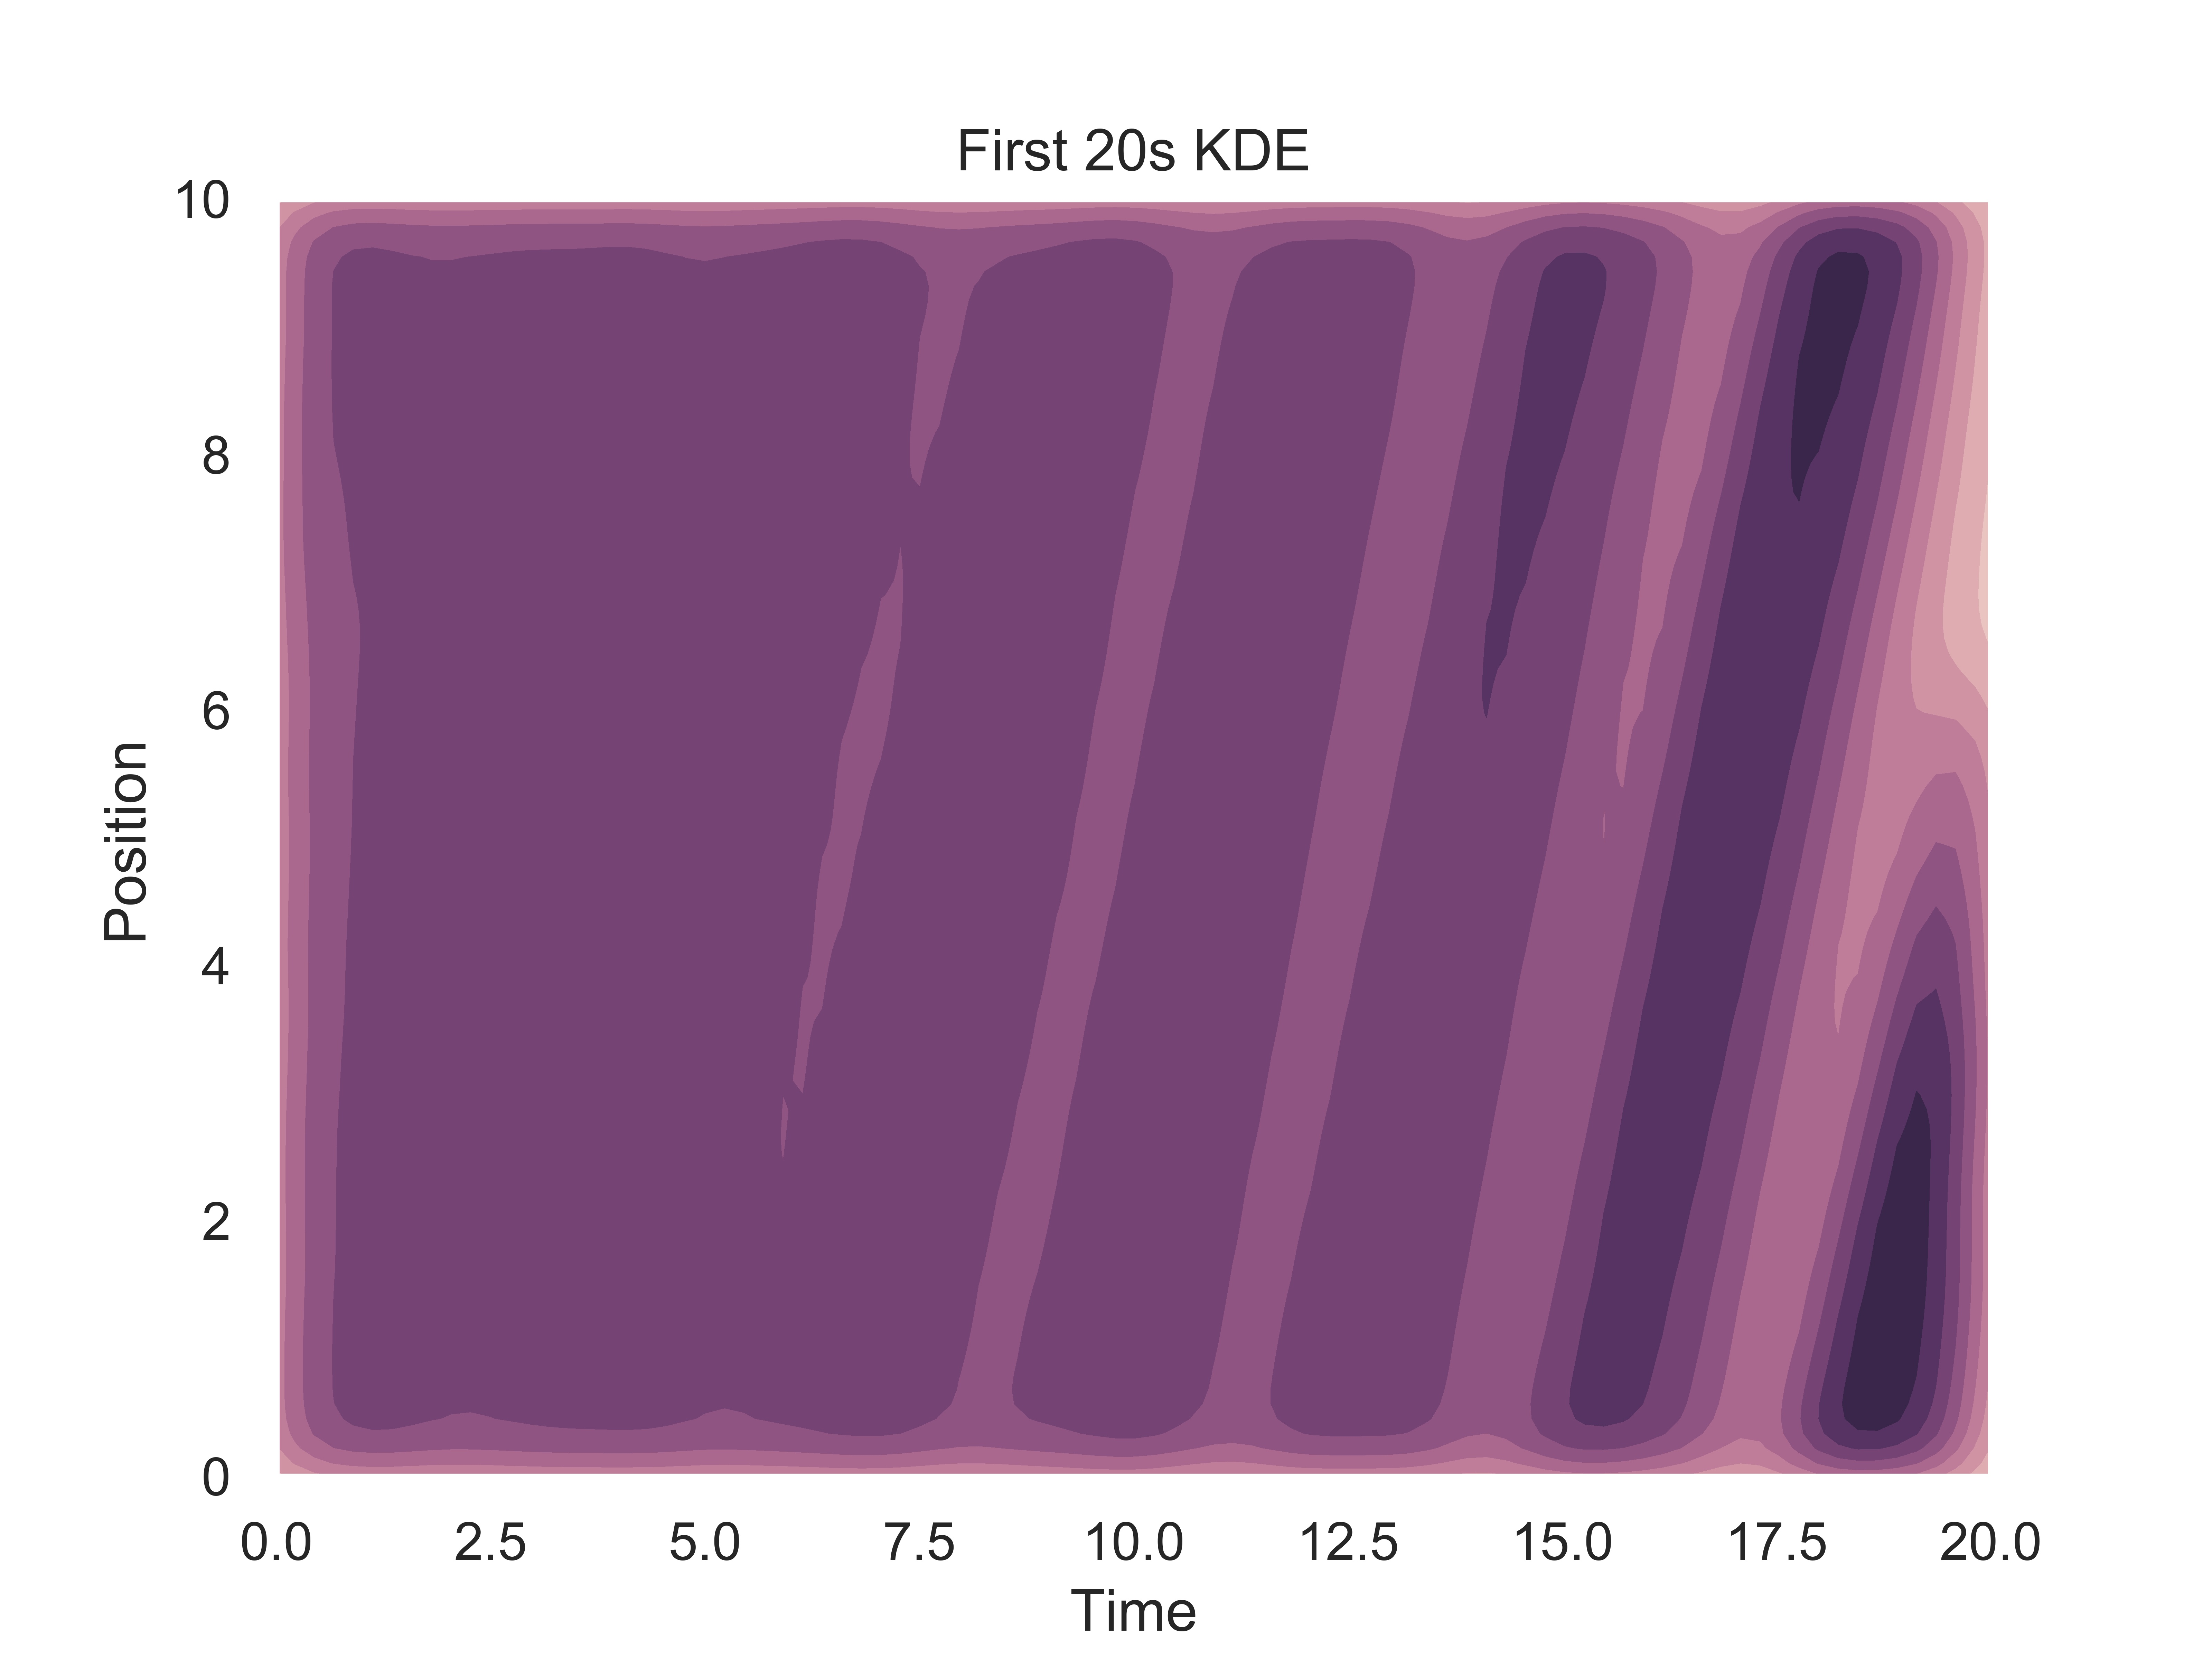
\includegraphics[width=\textwidth]{GarnierFigure4b}
    \end{minipage} %
    \begin{minipage}[b]{0.49\textwidth}
        \centering                    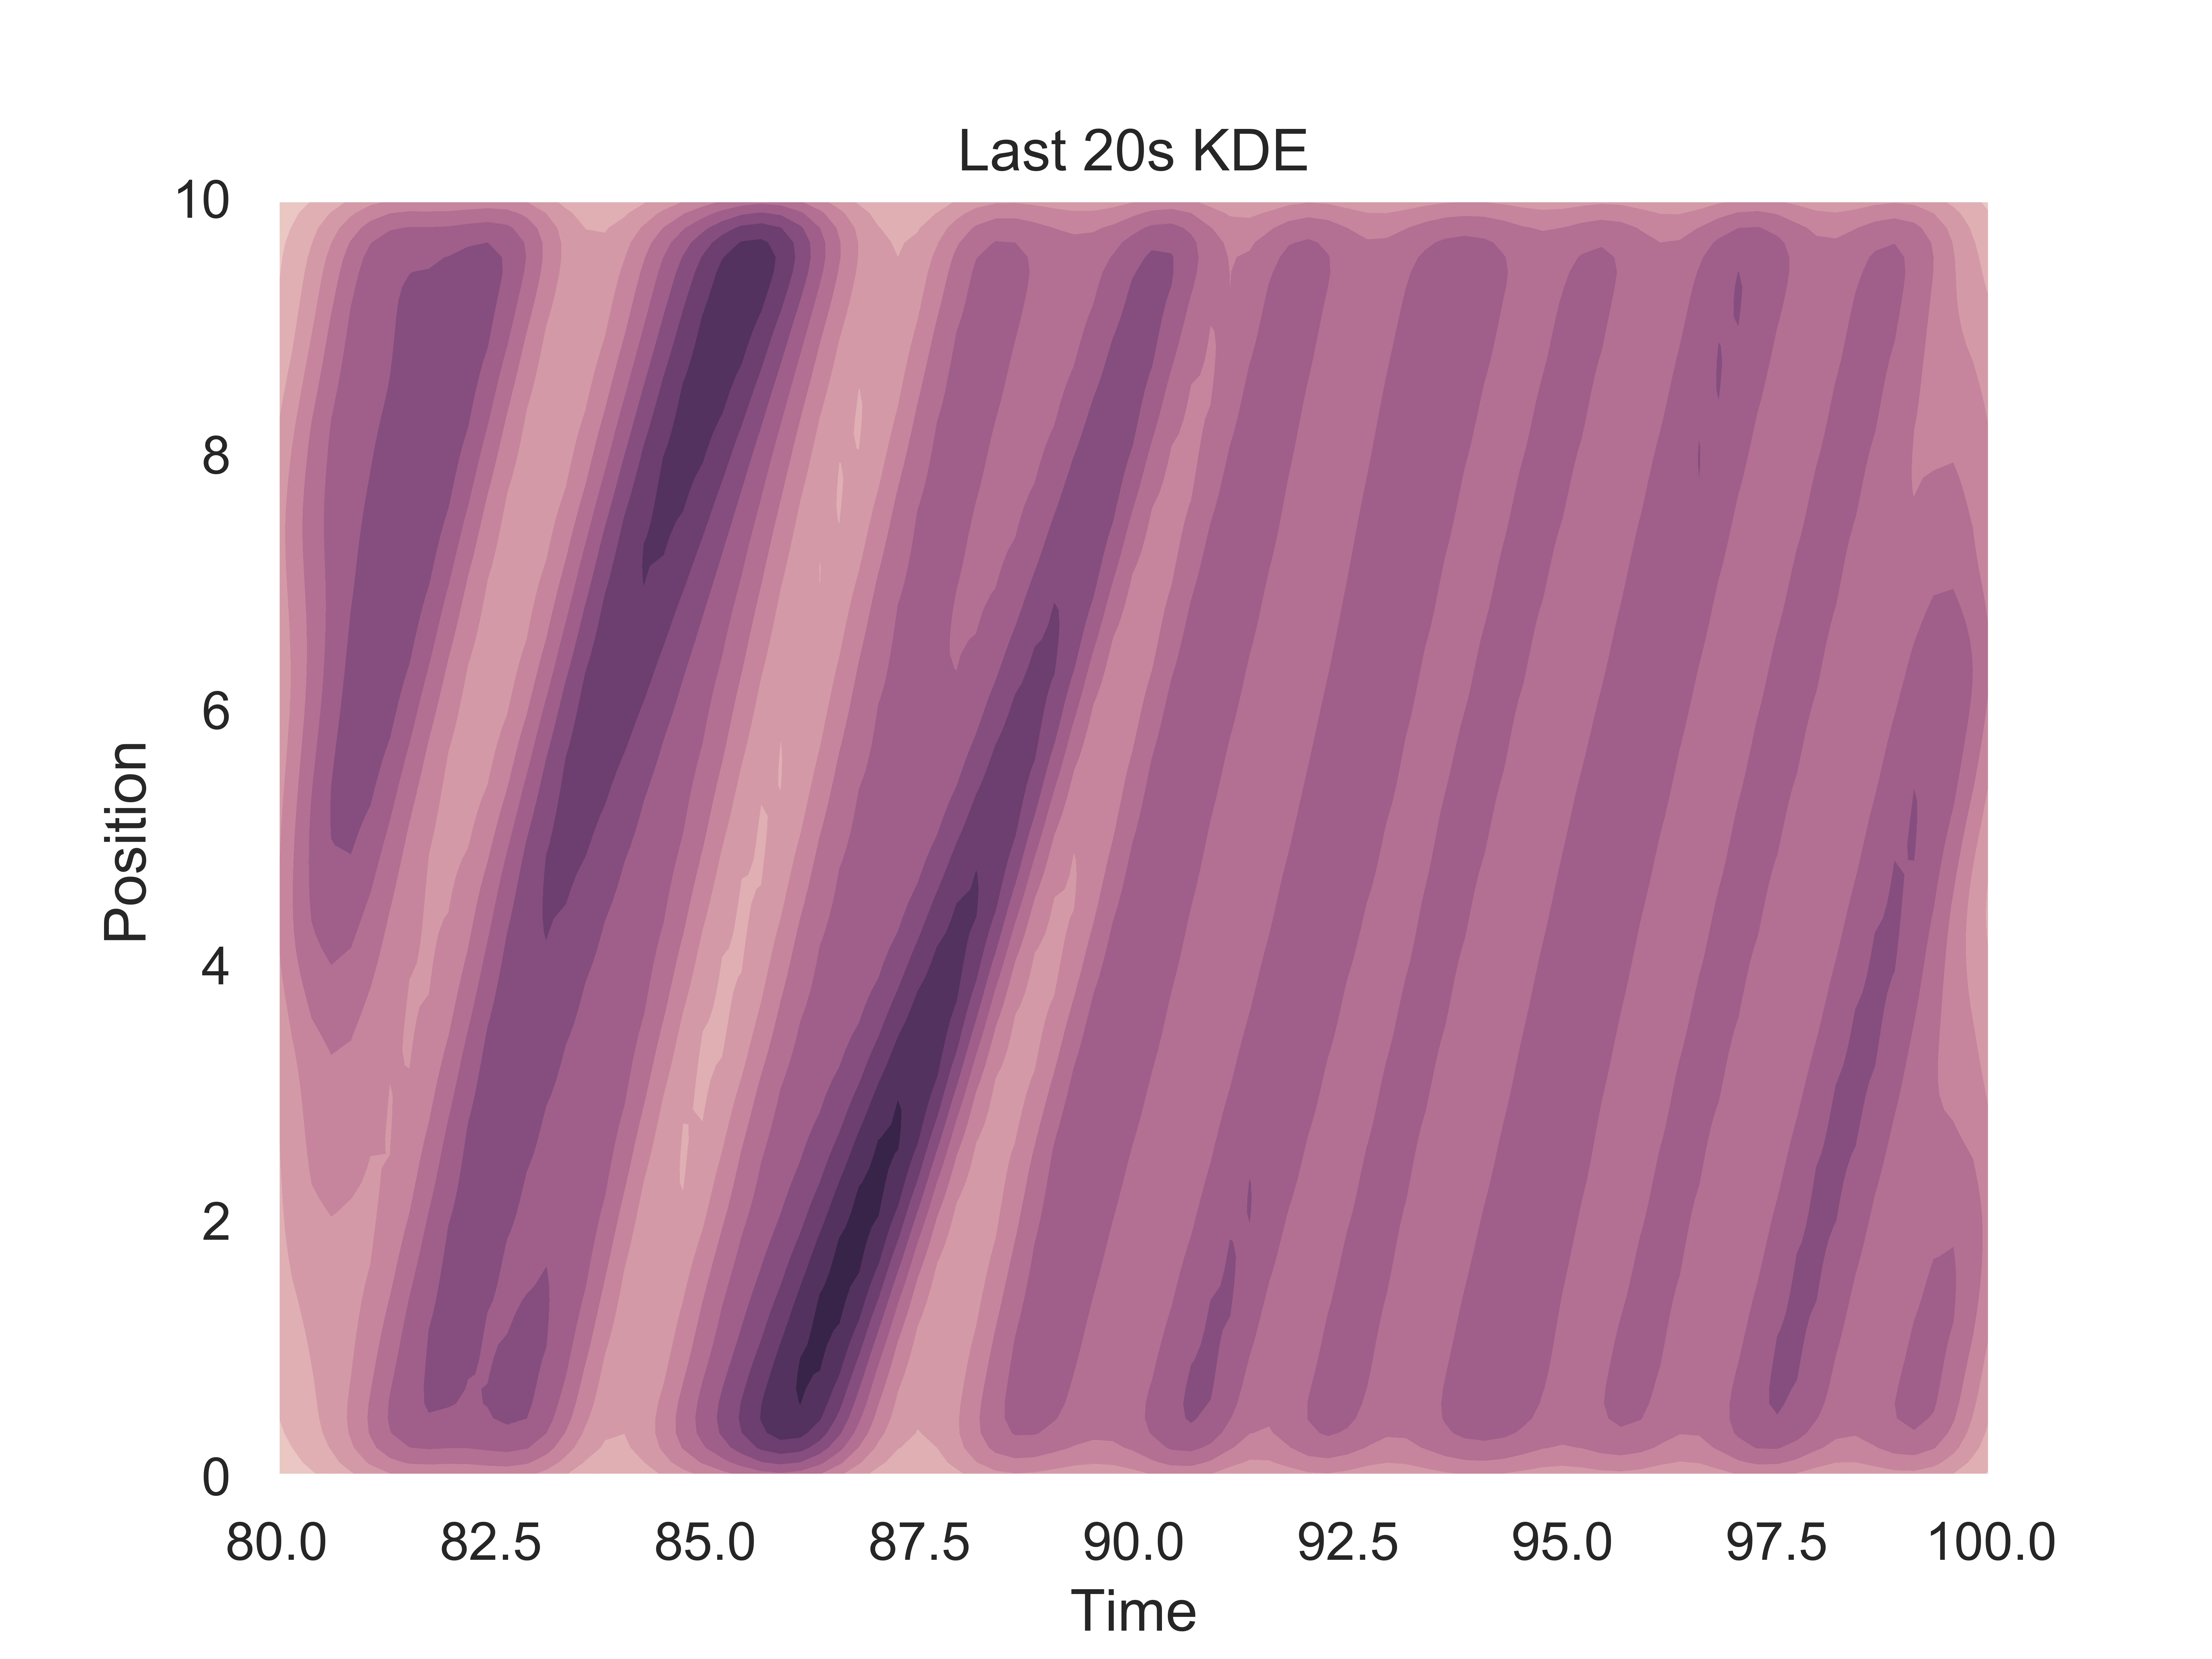
\includegraphics[width=\textwidth]{GarnierFigure4d}
    \end{minipage}
    \caption{Garnier Figure 4: Clusters occurring at low noise from stationarity. KDE Plots are harder than you'd think to place on a grid. Agrees with Garnier's result, although looks like the cluster is dissipating towards the end. A few more runs might show some transience, or a KDE plot for the whole 100s. The cluster could be forming and dissipating.}
\end{figure}

\begin{figure}
    \centering
    \includegraphics[width=1.1\linewidth]{GarnierFigure5}
    \caption{Garnier Figure 5: Clusters occurring at low noise. Setup is identical to GFig 3, but initial data for velocity has mean 0. Very similar to Garnier's result.}
    \end{figure}
    
    \begin{figure}
    \centering
    \begin{minipage}[b]{\textwidth}
        \centering
        
        \includegraphics[width=\textwidth]{GarnierFigure6}
    \end{minipage} \\
    
    \begin{minipage}[b]{0.49\textwidth}
        \centering
        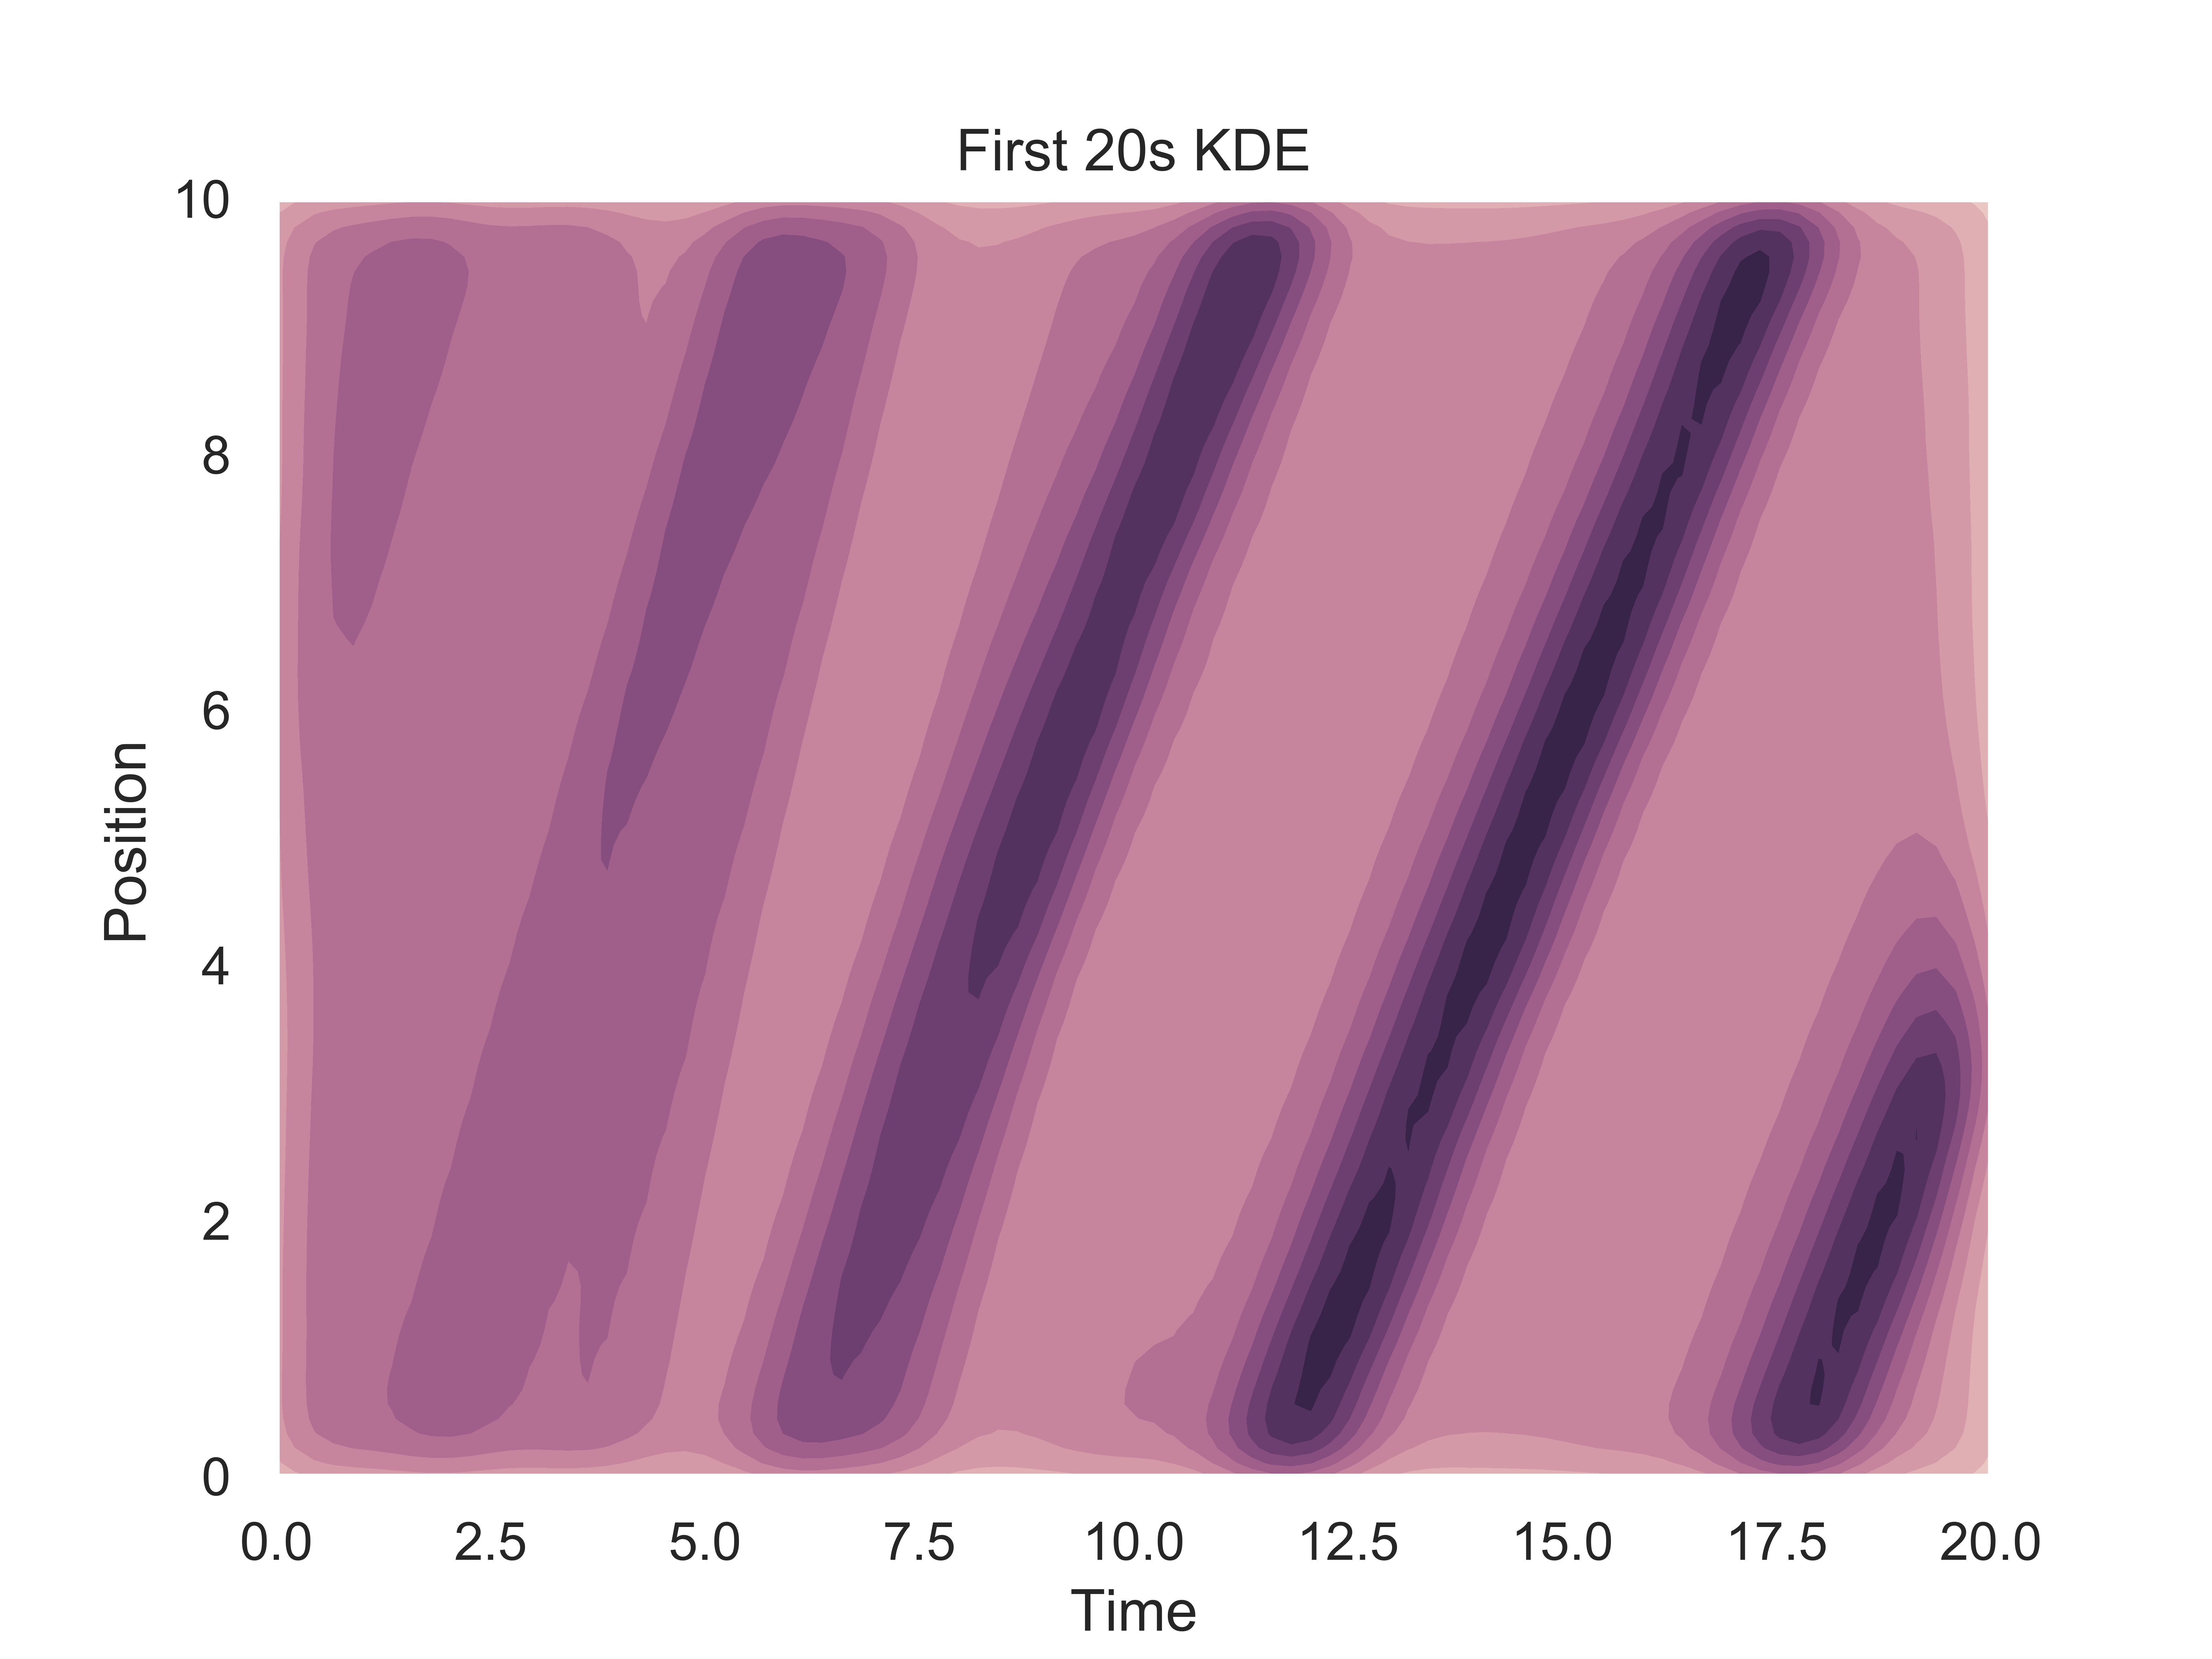
\includegraphics[width=\textwidth]{GarnierFigure6b}
    \end{minipage} %
    \begin{minipage}[b]{0.49\textwidth}
        \centering                    
        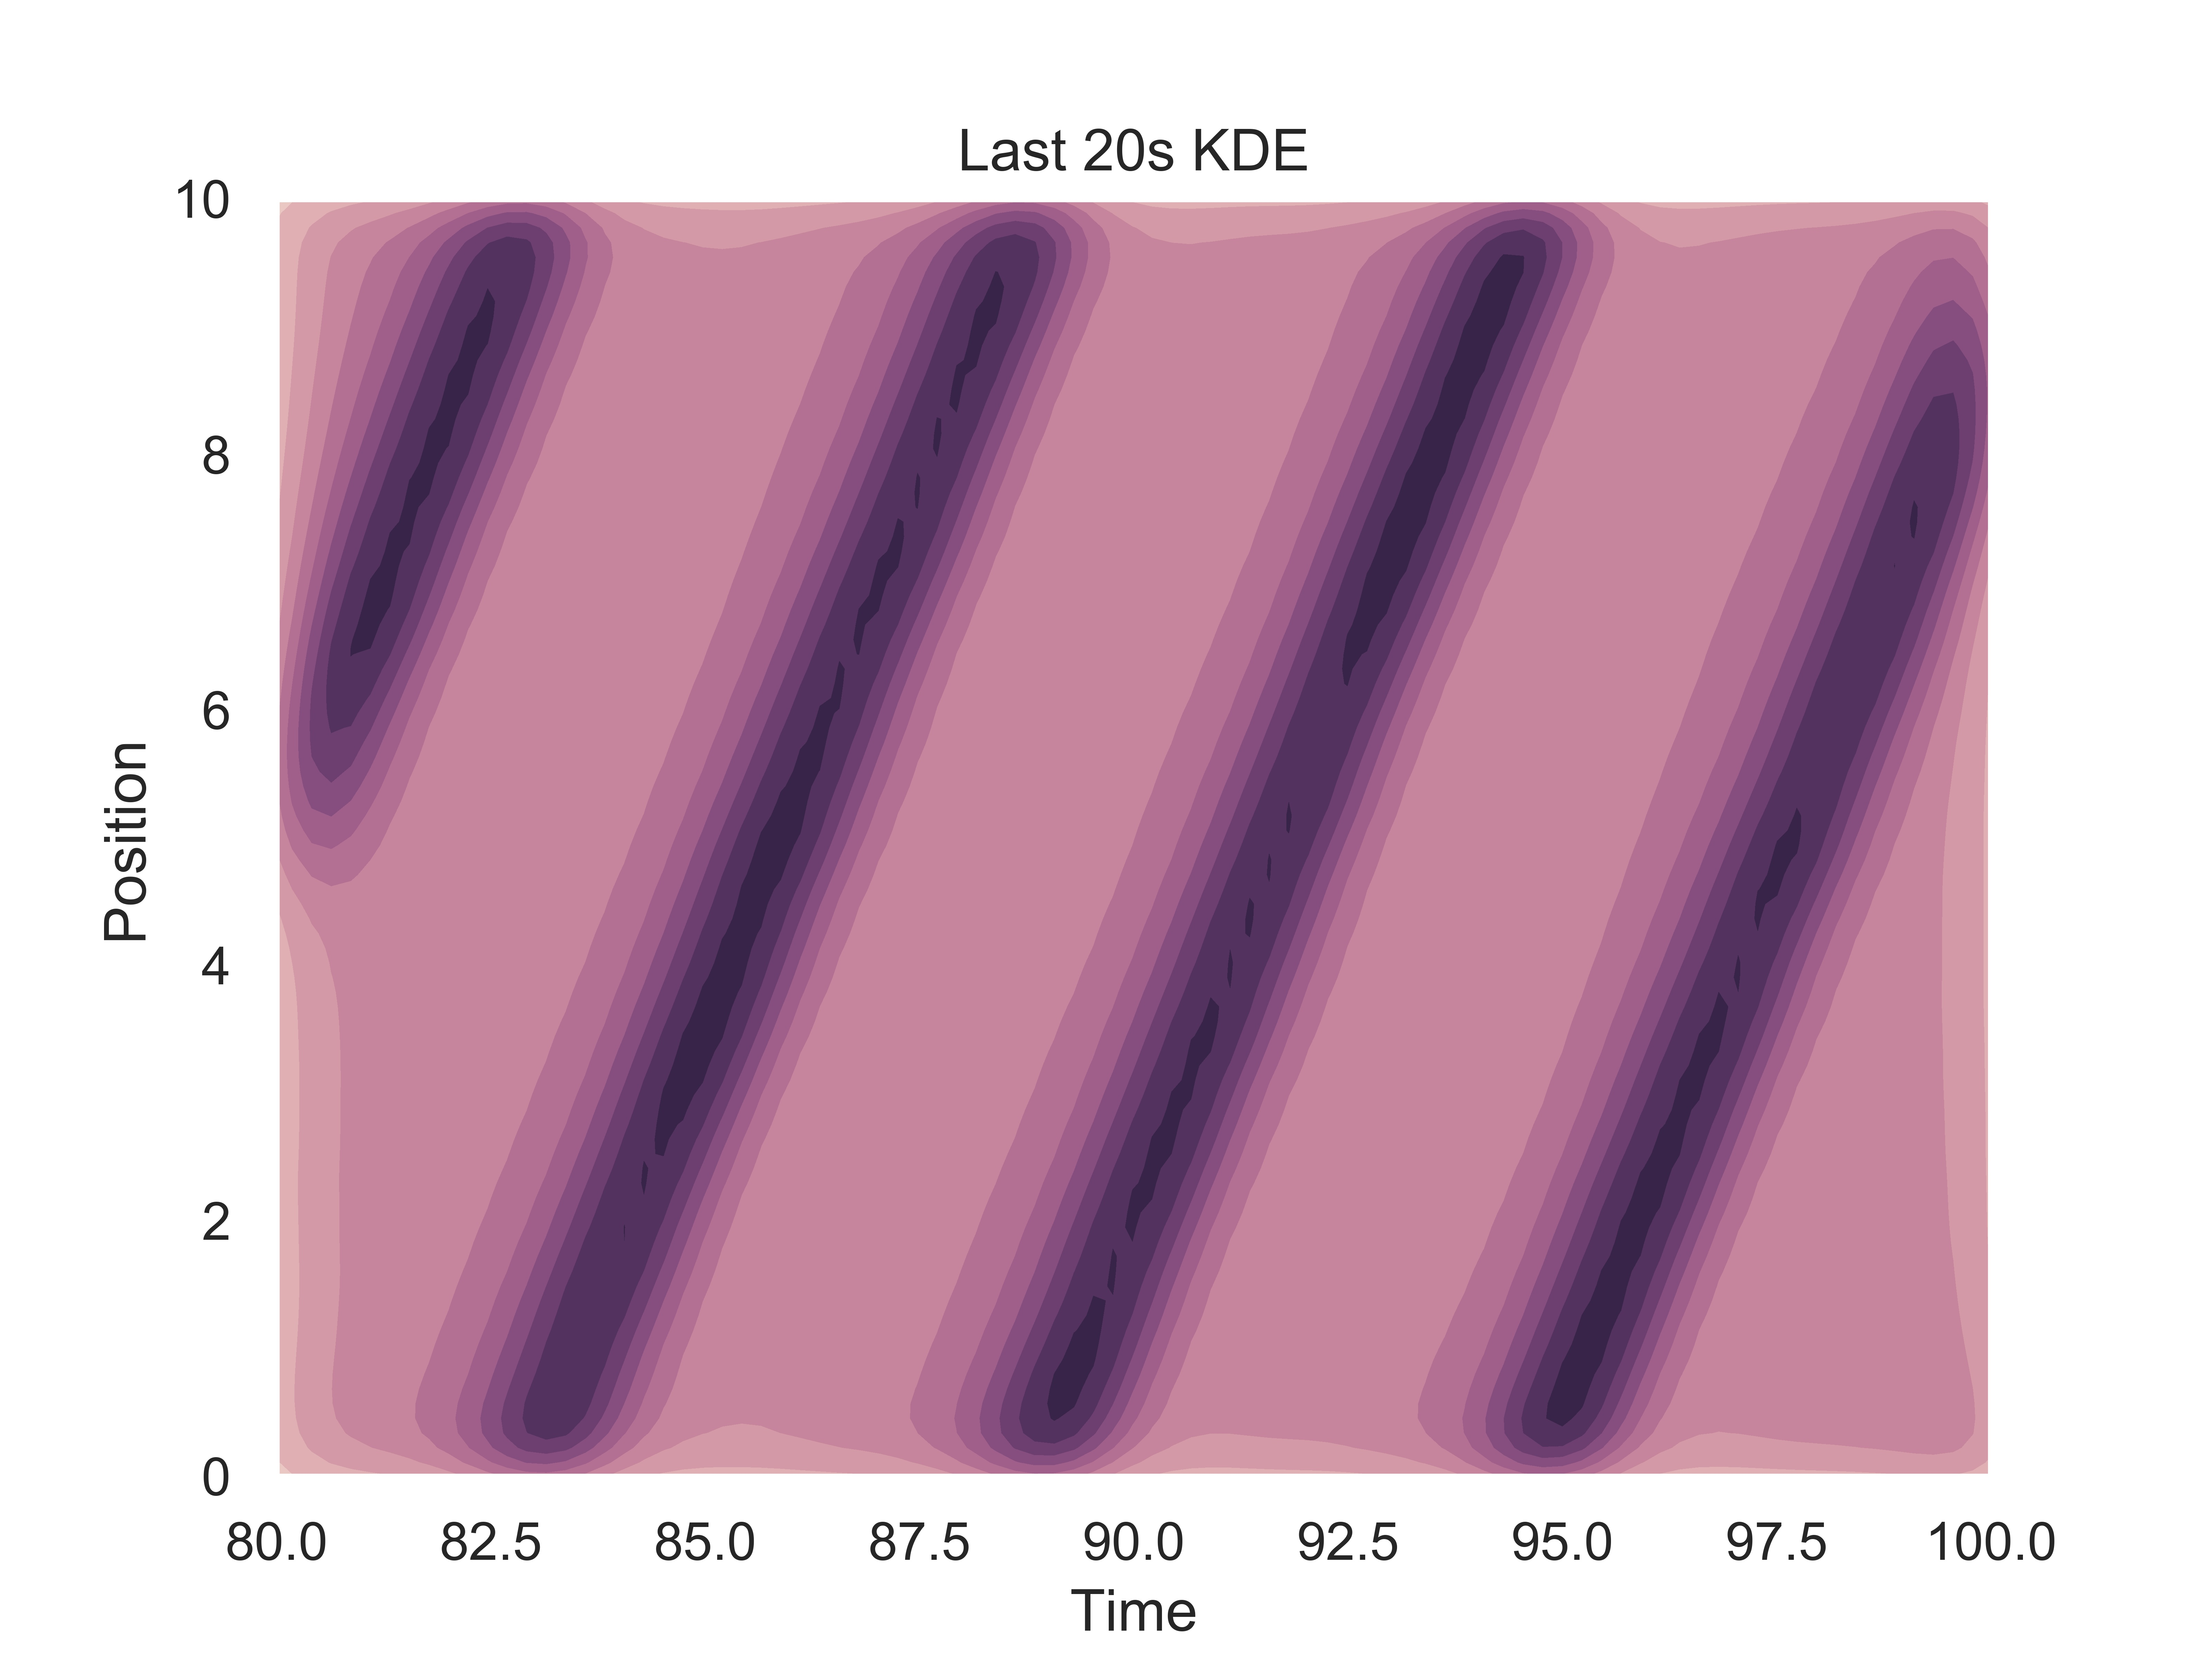
\includegraphics[width=\textwidth]{GarnierFigure6d}
    \end{minipage}
    \caption{Garnier Figure 6: Cluster forming out of stationarity. Well depth here is 10 and $\sigma = 1^2/2$. It is unclear how Garnier got a cluster forming here. +++COMPARE WITH GARNIER.+++}
\end{figure}
Figures 8, 9 and 10 are not particularly illuminating so I won't reproduce them.

\section{Experiments to try}
    How can we get clustering in our model? Can we show that it is transient?
\begin{itemize}
    \item Garnier parameters with proper weighted scaling like Butt\'a. Aim: show that lower avg velocity is artefact of scaling. (See below).
    \item Garnier parameters but with smooth/step $G$. Aim: convert Garnier's results to our model.
    \item Garnier parameters but smaller timestep/less particles/longer time. Aim: show clustering is transient.
    \item Implement interaction that gets stronger the further away particles are. Zero, Linear, Quadratic, etc. Aim: Force clustering, something Jakub said might work as similar things do for fractional Laplacian.
    \item Start with non-uniform distribution in space. Aim: show that clusters can be preserved.
    \item ???
\end{itemize}

\subsection{Scaling Garnier with Number of Particles Interacting }
Here we reproduce the Garnier figures but with the scaling of the interaction equal to the number of particles that the current particle interacts with, instead of the total number of particles. Garnier calls this $N_i$ and mentions it in Section 8. I think the effect will be to speed up any changes as the interaction is stronger at every step ($G$ is increasing, scaling by the number of particles reduces the change in velocity from interaction). Is this why clusters appear in Garnier? They randomly form and dissipate, but this happens too quickly when scaled properly?
\begin{figure}
    \centering
        \includegraphics[width=1.1\linewidth]{GarnierFigure2scaled}
    \caption{As in Garnier Figure 2 but scaled: Average velocity and CL2 discrepancy for $ h=2$ (top) and $h=4$ (bottom). This is pretty much identical to Garnier's, nothing interesting here. }
\end{figure}
\begin{figure}
    \centering
    \includegraphics[width=1.1\linewidth]{GarnierFigure3scaled}
    \caption{As in Garnier Figure 3 but scaled: Average velocity and CL2 discrepancy for $\sigma = 0.5^2/2$ (top), $\sigma = 1^2/2$ (middle) and $\sigma = 1.5^2/2$ (bottom). No clusters form! Perhaps check a noise even lower? Although $\sigma < 0.125$ is basically deterministic. Check deterministic?}
\end{figure}

\subsection{Interesting Bits}
Cluster forming when $\sigma =1^2/2$ in Figure 4.
\end{document}